%!TEX root = ../thesis.tex

\section{数値実験}
\label{part:experience}

本章では数値実験を行い、定義\ref{prop_model}による提案モデルが
前章で提案したAlgorithm 1によって推定可能であることを示す。
また、Algorithm 1による提案モデルの推定精度が、既存のDAG推定アルゴリズムより高いことを示す。
最後に、離散変数の因果順序を推定する際の閾値の設定に関しても考察する。
%
%!TEX root = ../thesis.tex

\subsection{設定}
\label{subsection:setup}

本論文では、サンプルサイズ$n = \{ 100, 250, 500, 1000, 1500, 2000, 2500 \}$、
頂点数$p = \{ 5, 10 \}$、
連続変数の誤差変数の分布 \{正規分布, 一様分布\} であるデータセットを、
提案モデルに従ってそれぞれ100個ずつ生成した。
その他のデータ生成や推定における設定の詳細は以下とした。

\begin{enumerate}
  \setlength{\itemsep}{0.3cm}
  \item
  $p$個の変数をランダムに連続変数と離散変数に割り当てた。
  連続変数に割り当てられる確率は0.6、離散変数に割り当てられる確率は0.4とした。
  また、離散変数はポアソン分布と二項分布のいずれかに確率0.5で割り当てた。
  ただし、二項分布のパラメータは
  Park and Raskutti(2017)\cite{Park2017-hw}と同様に$N_j=4$に固定した。

  \item
  グラフの構造をランダムに生成するために、
  まず全ての要素が0である$p\times p$隣接行列を生成した。
  次に、Kalisch and B\"{u}hlmann(2007)\cite{Kalisch2007-xg}と同様に、
  成功確率$s$に従う独立なベルヌーイ試行に基づいて
  隣接行列の下三角成分を1に置き換えた。
  成功確率$s$は、各変数と隣接する変数の個数の期待値が2または5になるように
  ランダムに設定した
  \footnote{各変数と隣接する変数の個数の期待値は$s(p-1)$である\cite{Kalisch2007-xg}}。
  隣接行列のゼロ・非ゼロパターンは、
  提案モデルにおける変数間の関係性の強さを表すパラメータ$\theta_{jk}$の
  ゼロ・非ゼロパターンと同じである。

  \item
  提案モデルにおける非ゼロのパラメータ$\theta_{jk} \in \mathbb R$は、
  範囲$\theta_{jk} \in [-0.5,-0.2]\cup [0.2,0.5]$の一様分布から選択した。
  また、定数項$\theta_j$は、範囲$\theta_j \in [-0.5,0.5]$の一様分布から選択した。

  \item
  連続変数のデータ生成過程における誤差変数の分散$\sigma_j^2$は、
  範囲$\sigma_j^2 \in [0.7,0.8]$の一様分布から選択した。

  \item
  離散変数の因果順序を推定する際の閾値は1.01とした。

  \item
  各変数の親変数との関係性の強さを推定する際の
  adaptive Lassoの調整パラメータについて、
  $\lambda$は10分割交差検証によって選択した。
  具体的には、「最小の逸脱度(deviance) +標準誤差」を超えない
  最大の$\lambda$を選択した。
  また、$\gamma$は1に固定した。
\end{enumerate}

既存のDAG推定アルゴリズムには、
Greedy Equivalent Search (GES)\cite{Chickering2002-iq}、
Max-Min Hill-Climbing (MMHC)\cite{Tsamardinos2006-qe}、
DirectLiNGAM\cite{Shimizu2011-pd}、
を用いた。
DAGを推定するアルゴリズムは、制約に基づくアプローチ(constraint-based approach)と
スコアに基づくアプローチ(score-based approach)に大別される。
GESはスコアに基づくアプローチであり、
ベイズ情報量規準(Bayesian Information Criterion; BIC)を用いて
モデルの当てはまりが最も良いマルコフ同値類を推定する方法である。
MMHCは制約に基づくアプローチとスコアに基づくアプローチの両方を組み合わせた
ハイブリッドなアルゴリズムである。
具体的には、まず制約に基づくアプローチによって各変数の親候補と子候補を求め、
次にスコアに基づくアプローチによってモデルの当てはまりが最も良いマルコフ同値類を推定する。
1段階目として制約に基づくアプローチによって親候補と子候補を求めることによって、
2段階目のスコアに基づくアプローチの際の探索空間を小さくしていることが特徴である。
DirectLiNGAMはLiNGAM\cite{Shimizu2006-yu}に特化したアルゴリズムであり、
回帰分析と独立性の評価を繰り返すことによって因果順序を推定する。

DAGの推定精度は、適合率(precision)と再現率(recall)によって測定した。
適合率と再現率の算出方法は以下の通りである。
\begin{itemize}
  \item 適合率(precision)
  \begin{equation*}
    \frac{\text{正しく推定された辺の個数}}{\text{推定されたDAGにおける辺の個数}}
  \end{equation*}

  \item 再現率(recall)
  \begin{equation*}
    \frac{\text{正しく推定された辺の個数}}{\text{真のDAGにおける辺の個数}}
  \end{equation*}
\end{itemize}
ただし、GESとMMHCはマルコフ同値類を推定するアルゴリズムであるため、
推定されたグラフの一部の辺は無向辺のままである。
そのため、本論文ではPark and Park(2019)\cite{Park2019-qy}と同様に、
推定されたマルコフ同値類すべてにおける適合率と再現率の平均値で評価する。

%
%!TEX root = ../thesis.tex

\subsection{結果}

各アルゴリズムのDAGの推定精度を図\ref{fig:plot_gaussian}
と\ref{fig:plot_uniform}に示す。
図\ref{fig:plot_gaussian}は
連続変数の誤差変数が正規分布に従うように生成したデータにおける推定精度を、
図\ref{fig:plot_uniform}は一様分布に従うように生成したデータにおける推定精度を示す。

実験結果より、提案アルゴリズムは他のアルゴリズムと比較して適合率も再現率も高いことが分かる。
また、提案アルゴリズムは他のアルゴリズムと比較して、サンプルサイズが大きくなるほど
有向辺の向きを正しく推定していることが分かる。
このことから、提案モデルは識別可能であり、本論文による提案アルゴリズムによって推定可能であると言える。
一方、DirectLiNGAMの推定精度は、正規分布の場合は適合率も再現率も0.5を下回るのに対し、
一様分布の場合はGESやMMHCの精度と同程度またはそれ以上である。
これは、LiNGAM\cite{Shimizu2011-pd}が誤差変数に対して非正規性を
仮定していることが影響しているためであると考えられる。

提案アルゴリズムにおける適合率と再現率を比較すると、
サンプルサイズが1000を超えると再現率のほうが高いことが読み取れる。
つまり、サンプルサイズが大きい時、
実際には直接的な因果関係があるにもかかわらず因果関係が無いと推定してしまうという偽陰性が少ない
ことを示している。
因果関係に関する仮説を得ようとする際に偽陰性が多いと、
重要な因果関係を見過ごしてしまう可能性が高まる。
そのため、因果関係の仮説を構築する上で、提案アルゴリズムの再現率が高いことは望ましいと言える。

\begin{figure}[H]
  \centering
  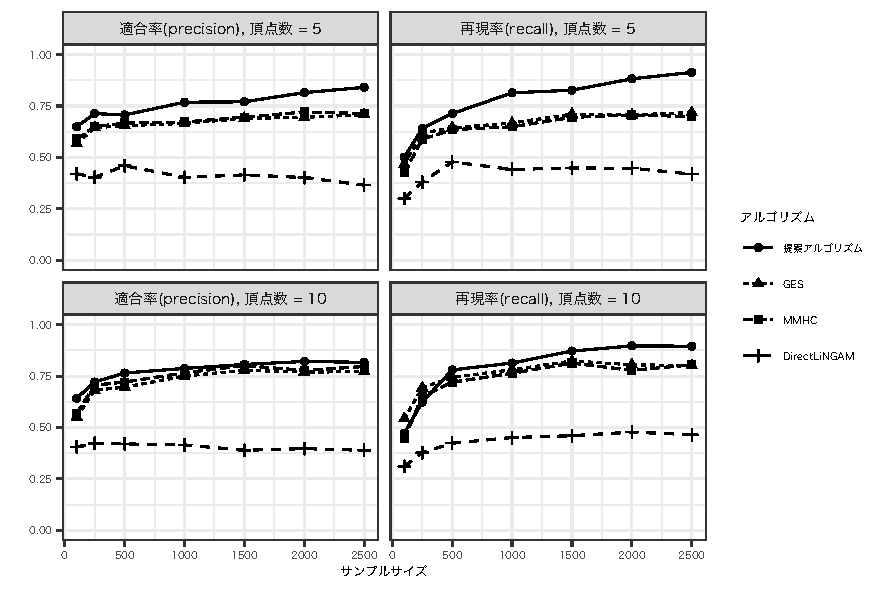
\includegraphics[width=13cm, bb=9 9 358 434]{./picture/plot_gaussian.pdf}
  \caption{連続変数の誤差変数が正規分布に従う提案モデルにおける各アルゴリズムの精度比較}
  \label{fig:plot_gaussian}
\end{figure}

\begin{figure}[H]
  \centering
  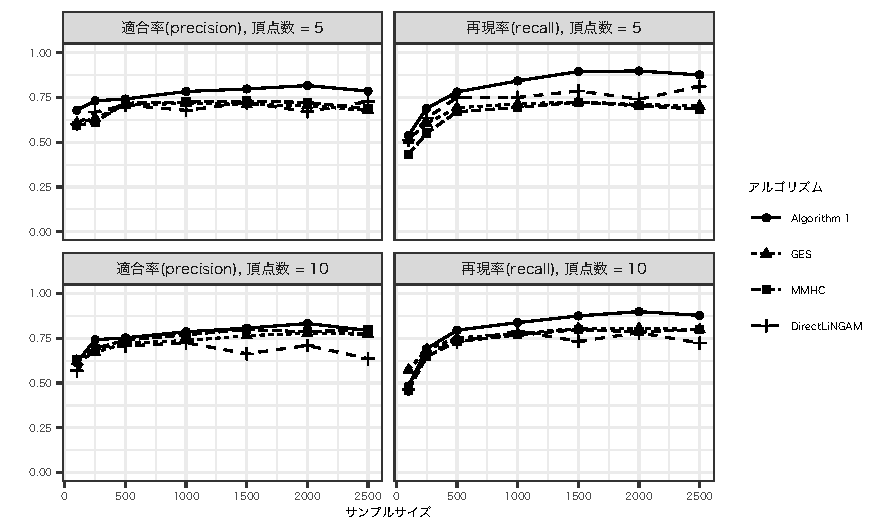
\includegraphics[width=13cm, bb=9 9 358 434]{./picture/plot_uniform.pdf}
  \caption{連続変数の誤差変数が一様分布に従う提案モデルにおける各アルゴリズムの精度比較}
  \label{fig:plot_uniform}
\end{figure}

%
%!TEX root = ../thesis.tex

\subsection{閾値の設定について}

閾値の設定について語るよ〜

